Tables \ref{table:results_base}–\ref{table:results_llmlingua} show the raw outcomes for the base method and the three proposed method. 

\begin{table}[htbp]
  \centering
  \caption{Token usage, API cost, and request count - Base Method}
  \begin{tabular}{
      l
      c@{\hspace{0.5em}}c@{\hspace{0.5em}}c@{\hspace{1em}}   % Claude   : Tokens ⟶ gap ⟶ Cost, Req.
      c@{\hspace{0.5em}}c@{\hspace{0.5em}}c@{\hspace{1em}}   % Gemini   : Tokens ⟶ gap ⟶ Cost, Req.
      c@{\hspace{0.5em}}c@{\hspace{0.5em}}c   % GPT-4.1 : Tokens ⟶ gap ⟶ Cost, Req.
    }
    \toprule
          & \multicolumn{3}{c}{Claude 3.7 Sonnet}
          & \multicolumn{3}{c}{Gemini 2.5 Pro Preview}
          & \multicolumn{3}{c}{GPT-4.1} \\
    \cmidrule(lr){2-4}\cmidrule(lr){5-7}\cmidrule(lr){8-10}
    Run & Tokens & Cost(USD) & Req. & Tokens & Cost(USD) & Req. & Tokens & Cost(USD) & Req. \\
    \midrule
    1 & 427\,000 & 0.418 & 16 & 353\,000 & 0.363 & 14 & 319\,000 & 0.230 & 13 \\
    2 & 559\,000 & 0.672 & 19 & 643\,000 & 0.457 & 22 & 454\,000 & 0.313 & 14 \\
    3 & 370\,000 & 0.381 & 14 & 498\,000 & 0.410 & 18 & 374\,000 & 0.236 & 15 \\
    4 & 436\,000 & 0.404 & 16 & 340\,000 & 0.285 & 14 & 433\,000 & 0.267 & 17 \\
    5 & 587\,000 & 0.635 & 19 & 491\,500 & 0.371 & 18 & 386\,000 & 0.246 & 15 \\
    \midrule
    Average\hspace{0.5em} & 475\,800 & 0.502 & 16.8 & 465\,100 & 0.3772 & 17.2 & 393\,200 & 0.258 & 14.8 \\
    \bottomrule
  \end{tabular}
  \label{table:results_base}
\end{table}



\begin{table}[htbp]
  \centering
  \caption{Token usage, API cost, and request count - Proposed Method 1}
  \begin{tabular}{
      l
      c@{\hspace{0.5em}}c@{\hspace{0.5em}}c@{\hspace{1em}}   % Claude   : Tokens ⟶ gap ⟶ Cost, Req.
      c@{\hspace{0.5em}}c@{\hspace{0.5em}}c@{\hspace{1em}}   % Gemini   : Tokens ⟶ gap ⟶ Cost, Req.
      c@{\hspace{0.5em}}c@{\hspace{0.5em}}c                 % GPT-4.1  : Tokens ⟶ gap ⟶ Cost, Req.
    }
    \toprule
          & \multicolumn{3}{c}{Claude 3.7 Sonnet}
          & \multicolumn{3}{c}{Gemini 2.5 Pro Preview}
          & \multicolumn{3}{c}{GPT-4.1} \\
    \cmidrule(lr){2-4}\cmidrule(lr){5-7}\cmidrule(lr){8-10}
    Run & Tokens & Cost(USD) & Req. & Tokens & Cost(USD) & Req. & Tokens & Cost(USD) & Req. \\
    \midrule
    1 & 751\,000 & 0.576  & 23 & 682\,000 & 0.780 & 24 & 301\,000 & 0.223 & 13 \\
    2 & 329\,000 & 0.348  & 14 & 296\,000 & 0.217 & 13 & 296\,000 & 0.217 & 13 \\
    3 & 546\,000 & 0.503  & 19 & 478\,000 & 0.360 & 19 & 363\,000 & 0.233 & 15 \\
    4 & 449\,000 & 0.595  & 18 & 485\,333 & 0.452 & 19 & 373\,000 & 0.231 & 16 \\
    5 & 743\,000 & 0.701  & 23 & 580\,000 & 0.570 & 22 & 300\,000 & 0.223 & 13 \\
    \midrule
    Average\hspace{0.5em} & 563\,600 & 0.5446 & 19.4 & 504\,267 & 0.476 & 19.2 & 326\,600 & 0.225 & 14.0 \\
    \bottomrule
  \end{tabular}
  \label{table:results_prompt_only}
\end{table}



\begin{table}[htbp]
  \centering
  \caption{Token usage, API cost, and request count - Proposed Method 2}
  \begin{tabular}{
      l
      c@{\hspace{0.5em}}c@{\hspace{0.5em}}c@{\hspace{1em}}
      c@{\hspace{0.5em}}c@{\hspace{0.5em}}c@{\hspace{1em}}
      c@{\hspace{0.5em}}c@{\hspace{0.5em}}c
    }
    \toprule
          & \multicolumn{3}{c}{Claude 3.7 Sonnet}
          & \multicolumn{3}{c}{Gemini 2.5 Pro Preview}
          & \multicolumn{3}{c}{GPT-4.1} \\
    \cmidrule(lr){2-4}\cmidrule(lr){5-7}\cmidrule(lr){8-10}
    Run & Tokens & Cost(USD) & Req. & Tokens & Cost(USD) & Req. & Tokens & Cost(USD) & Req. \\
    \midrule
    1 & 377\,000 & 0.361 & 15 & 350\,000 & 0.395 & 14 & 409\,000 & 0.285 & 16 \\
    2 & 371\,000 & 0.289 & 15 & 453\,000 & 0.401 & 17 & 312\,000 & 0.195 & 13 \\
    3 & 561\,000 & 0.494 & 19 & 401\,500 & 0.398 & 16 & 314\,000 & 0.196 & 13 \\
    4 & 430\,000 & 0.654 & 16 & 677\,000 & 0.621 & 23 & 671\,000 & 0.414 & 23 \\
    5 & 612\,000 & 0.540 & 20 & 565\,000 & 0.511 & 20 & 321\,000 & 0.204 & 13 \\
    \midrule
    Average\hspace{0.5em} & 470\,200 & 0.4676 & 17.0 & 489\,300 & 0.4652 & 17.9 & 405\,400 & 0.259 & 15.6 \\
    \bottomrule
  \end{tabular}
  \label{table:results_llmlingua}
\end{table}

% \begin{figure}[htbp]
    \centering
    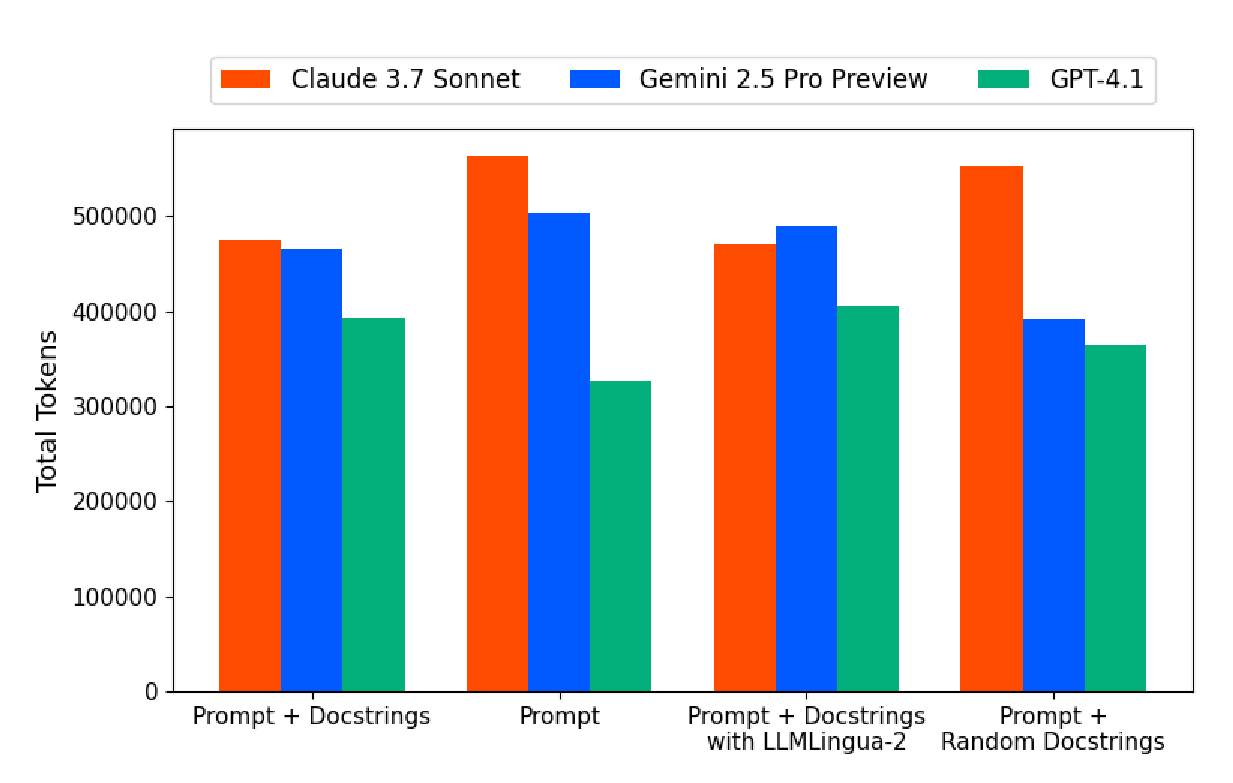
\includegraphics[width=0.9\linewidth]{imgs/eps/total_tokens_all.eps}
    \caption{Total Tokens}
    \label{fig:total_tokens}
\end{figure}

\begin{figure}[htbp]
    \centering
    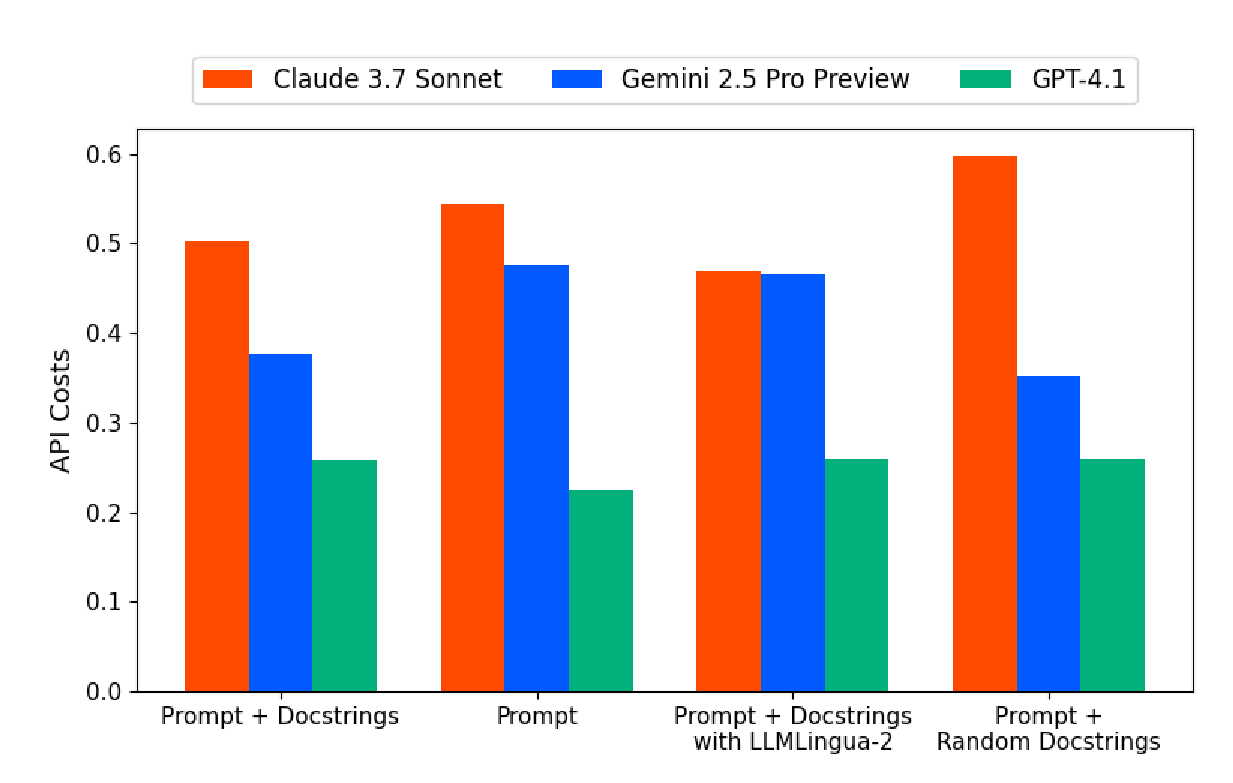
\includegraphics[width=0.9\linewidth]{imgs/eps/total_api_costs_all.eps}
    \caption{Total API Costs}
    \label{fig:total_api_costs}
\end{figure}

\begin{figure}[htbp]
    \centering
    \includegraphics[width=0.9\linewidth]{imgs/eps/total_requests_all.eps}
    \caption{Total Requests}
    \label{fig:total_requests}
\end{figure}

\newpage

\subsection{Quantitative Comparison about Token Counts and API Costs, Number of Requests}

Table \ref{table:quantitative_comparison} shows the difference (\%) from the base method calculated based on the average values in Table \ref{table:results_base}-\ref{table:results_llmlingua}. PM means Proposed Method.

\begin{table}[h!]
    \centering
    \caption{Change Rates of LLM Performance Metrics (Relative to Base Method)}
    \begin{tabular}{lcccc}
        \toprule
        \textbf{LLMs} & \textbf{Metrics} \quad & \textbf{Base Method} & \textbf{PM1} & \textbf{PM2} \\
        \midrule
        \multirow{3}{*}{Claude 3.7 Sonnet} 
          & Tokens & 475{,}800 & \quad +18.4\% & \quad $-1.2$\% \\
          & Cost   & \$0.502 & \quad +8.6\% & \quad $-6.8$\% \\
          & Req.   & 16.8 & \quad +2.6 & \quad +0.2 \\
        \midrule
        \multirow{3}{*}{Gemini 2.5 Pro Preview} 
          & Tokens & 465{,}100 & \quad +8.4\% & \quad +5.2\% \\
          & Cost   & \$0.377 & \quad +26.2\% & \quad +23.3\% \\
          & Req.   & 17.2 & \quad +2.0 & \quad +0.7 \\
        \midrule
        \multirow{3}{*}{GPT-4.1} 
          & Tokens & 393{,}200 & \quad $-17.0$\% & \quad +3.1\% \\
          & Cost   & \$0.258 & \quad $-12.8$\% & \quad +0.4\% \\
          & Req.   & 14.8 & \quad $-0.8$ & \quad +0.8 \\
        \bottomrule
    \end{tabular}
    \label{table:quantitative_comparison}
\end{table}

Table \ref{table:impact_of_each_method} shows a summary of the performance impact of each proposed method from Table \ref{table:quantitative_comparison}. From Table \ref{table:impact_of_each_method}, we can see these things:

\begin{enumerate}
    \item \textbf{LLMs Dependency}
        \begin{itemize}[label={$\bullet$}]
            \item Claude 3.7 Sonnet and Gemini 2.5 Pro Preview rely heavily on Docstrings for code understanding. Removing them leads to more correction requests.
            \vspace{0.2cm}
            
            \item GPT-4.1 shows low dependence on Docstrings and may even treat them as a source of noise.
        \end{itemize}
\vspace{0.3cm}

    \item \textbf{LLMLingua-2 Compression as a “Safe Option”}
        \begin{itemize}[label={$\bullet$}]
            \item Produced the best results with Claude 3.7 Sonnet. With Gemini 2.5 Pro Preview and GPT-4.1, the changes were minor, and the quality (Req) was largely maintained.
            \vspace{0.2cm}
            
            \item Since there’s little risk of degradation, it is effective as a general-purpose prompt-engineering strategy for reducing API costs.
        \end{itemize}
\end{enumerate}

\begin{table}[ht]
  \centering
  \caption{Impact of Each Method on Token Usage, Cost, and Request Count (relative to base method)}
  \setlength{\tabcolsep}{8pt}         % horizontal padding per column
  \begin{tabularx}{\linewidth}{@{}l L L@{}}  % ← Y → L
    \toprule
    \textbf{LLMs} &
    \thead{PM 1\\Docstrings Removal} &
    \thead{PM 2\\LLMLingua-2 Compression} \\
    \midrule
    Claude &
    \hspace{1.8cm} \makecell[l]{
      $\times$ Tokens/ Cost/ Req \textbf{increase}\\[2pt]
      $\Rightarrow$ All metrics degraded
    } &
    \hspace{2.0cm} \makecell[l]{
      $\bigcirc$ Tokens $-1.2\%$\\
      $\bigcirc$ Cost $-6.8\%$\\
      $\triangle$ Req $\approx$ unchanged\\[2pt]
      $\Rightarrow$ \textbf{lowest cost}
    } \\
    \addlinespace[4pt]
    \midrule[0.2pt] 
    Gemini &
    \hspace{1.8cm} \makecell[l]{
      $\times$ All metrics degraded
    } &
    \hspace{2.0cm} \makecell[l]{
      $\times$ All metrics degraded
    } \\
    \addlinespace[4pt]
    \midrule[0.2pt] 
    GPT-4.1 &
    \hspace{1.8cm} \makecell[l]{
      $\bigcirc$ Tokens $-17\%$\\
      $\bigcirc$ Cost $-12.8\%$\\
      $\bigcirc$ Req slightly \textbf{reduce}\\[2pt]
      $\Rightarrow$ \textbf{overall best} for GPT-4.1
    } &
    \hspace{2.0cm} \makecell[l]{
      $\triangle$ Roughly identical to \\ \hspace{0.5cm}base method
    } \\
    \bottomrule
  \end{tabularx}
  \label{table:impact_of_each_method}
\end{table}


\subsection{Code Coverage}
Under all conditions, the generated test cases achieved 100\% code coverage, as measured using the Pytest library. This result indicates that, at least for the dataset used in this study, neither the presence nor absence of natural language information—nor its compression—affected the final coverage.

\subsection{Impact of Docstrings}
Figure \ref{fig:token_usage_comparison} shows token usage statistics—mean, variance, minimum, and maximum—comparing the Base Method and Proposed Method 1 (Docstrings removed). For Claude 3.7 Sonnet, removing Docstrings reduces the variability in token counts, indicating more stable outputs without in-code descriptions. In contrast, Gemini 2.5 Pro Preview and GPT-4.1 show little change in variability, whether Docstrings are present or not.

Figure \ref{fig:variablity_comparison} presents the coefficient of variation (CV), which normalizes spread relative to scale. CV can calculated by standard deviation ($\sigma$) divided by the mean ($\mu$) as shown below. Here, Claude’s coefficient jumps significantly when Docstrings are omitted, revealing its strong dependence on Docstrings for consistent code comprehension. Meanwhile, Gemini 2.5 Pro Preview and GPT-4.1 maintain low and nearly identical coefficients across both conditions, suggesting that Docstrings have minimal impact on their understanding and output stability.

\[
\mathrm{CV} = \frac{\sigma}{\mu}
\]

\begin{figure}[htbp]
    \centering
    \includegraphics[width=1.0\linewidth]{imgs/eps/token_usage_comparison.eps}
    \caption{Token Usage Comparison: Mean Values with Standard Deviation}
    \label{fig:token_usage_comparison}
\end{figure}



\begin{figure}[htbp]
    \centering
    \includegraphics[width=1.0\linewidth]{imgs/eps/variability_comparison.eps}
    \caption{Variability Comparison: Coefficient of Variation}
    \label{fig:variablity_comparison}
\end{figure}
